\chapter{Background}
\label{chap:technical}

I begin by discussing the technical background that relates to the work in the dissertation, to provide a foundation from which to build the rest of the project.

\section{Sentiment Analysis}
Sentiment analysis (also known as opinion mining) is the task of identifying opinions or sentiment of authors from an input of text. The implications of being able to programmatically extract the intended meaning of an input are profound and its application could prove valuable in a variety of fields, especially in a financial context. The nuances of natural language can sometimes make this difficult to extract, and therefore significant research has been conducted on the topic throughout previous decades.

The success or failure of any approach to this task can be summarised as the closeness of a prediction of sentiment to that calculated by a human. Take, for example, the following sentences:

\begin{enumerate}
\item \textit{`The movie was great'}
\item \textit{`The movie was terrible'}
\item \textit{`The acting was terrible, but the movie was great'}
\end{enumerate}

Sentences 1 and 2 have very simple sentiment: one is positive, and the other is negative. However, sentence 3 has slightly more complex sentiment. If the feature of interest is the movie, the word \textit{`terrible'} does not influence the sentiment of this feature as it is used in reference to the acting. Simpler analysis methods may not pick up on such nuances in language.

\subsection{Pre processing}
Here, I introduce three terms used in the pre-processing of text data. The main goal of pre-processing in sentiment analysis is to ensure sentiment is being assigned to the correct words. Stop words are a term used in NLP to describe very commonly used words that are considered unimportant (such as `and' or `the'). They serve only as noise and are removed to focus on more impactful words. 

Stemming and lemmatisation are two techniques whose primary is to reduce different forms of a word to its common base form. For example, `am, are, is' all become `be' as it is the root of the word \parencite{stem-lem}. The two techniques share a common goal, but achieve this in different ways. Stemming refers to a more crude process that is effective at the potential cost of precision. In general, it consists of applying a series of rules sequentially, each of which reducing a word. For each reduction, there are conventions to select certain rules. There are a variety of stemmers that each perform stemming in a unique way. On the other hand, lemmatisers are a tool from NLP that does analysis to identify the \textit{lemma}, or the language word root. Both techniques have advantages and disadvantages and as a result the two are often used in tandem, as they compliment one another.

The textual input to any sentiment analysis algorithm requires high quality preprocessing to ensure that the data is of the same format, and is one of the primary steps in any technique. Keeping noisy features such as stop words, or HTML tags serves to muddy the output. Instead, only features of interest should be considered in the ideal scenario \parencite{haddi2013preprocessing}. Insufficient data pre-processing can lead to underachieving analysis models, and as such the importance of this step should not be overlooked. Traditionally, this consists of online text cleaning (if necessary), removal of stop words and whitespace, and stemming and lemmatisation.

\subsection{Lexicon Based Methods}
The fundamental concept of sentiment analysis revolves around investigating a piece of text and deciding on a binary classification: positive or negative. The simplest method involves compiling a weighted word list, known as a lexicon. The weight of a word corresponds to the associated positivity or negativity of the word (for example `great' would have a high positivity, while `terrible' would have a very high negativity score) \parencite{taboada2011lexicon}. The overall sentiment of a piece of text could then be estimated by summing the individual positive sentiment scores of each word while subtracting the negative sentiment scores to yield an overall score for a piece of text. This lexicon is not limited to single words, and can be expanded to include $n$-grams (phrases of $n$ words), as the context in which a word is used can dramatically change its sentiment. This may increase the accuracy of the dictionary at the cost of increased dimensionality. The lexicon itself must be compiled before it is possible to utilise this method, and is normally constructed via in-depth analysis of many texts. An example of a lexicon used for English text is the Harvard-IV-4 psychosociological lexicon (H4) which is a general usage model that can be used to estimate the sentiment of a piece of text.

Certain words that may have no meaning at all in one context, may have significant sentiment in another, particularly in the field of finance, where jargon dominates text. \textcite{lm-dict} conducted an investigation into the use of standard lexicons for analysing 10-K filing reports, which are comprehensive reports filed by companies about their financial performance. They discovered that almost 75\% of negative words found in the filings based on the H4N file were not typically negative in a financial context. For example, `liability' is a negatively charged word in a standard context, while it carries no tone at all in the context of the filings. Some words were found to have strong links to certain industry specific sectors, meaning they had no relevance without the context of a specific industry sector. Loughran and McDonald created their own lexicon based on these results called the Loughran McDonald dictionary specifically for the purpose of classifying 10-k filings. They find that there is a high misclassification rate when using these generic lexicons, proving lexicon based methods work far better if it is bespoke for the topic. 

There are many difficulties faced with creating a dictionary of this sort, as language is often a subjective entity, leading to conflicting opinions in assigning tone to a specific word. Furthermore, the context within which a word is used can drastically change the intended sentiment of a word. For example, the word `great' is naturally a very positive word, however, if used in a sarcastic manner (e.g. `It's so great that my flight is delayed!') the sentiment conveyed can be inverted entirely. For this reason, simply calculating the sentiment of a piece of text on a word by word level can give an incorrect estimate. Additionally, sentiment analysis is reliant on sufficiently labelled data and lack of this data is a significant obstacle in the field \parencite{madhoushi2015sentiment}.

\subsubsection{Usage}
Usage of these lexicons can vary greatly, with some simply summing the count of positive words and subtracting the count of negative words to end up with an overall word count leaning either positively or negatively. However, this is a very rudimentary method and can be augmented with more complex models. Loughran and McDonald themselves suggest using Term Frequency Inverse Document Frequency (TF-IDF) as a method to weight the word counts. TF-IDF is one of the most popular term weighting schemes, and it therefore makes sense to augment these strategies with this weighting.

TF-IDF has two distinct parts, term frequency and inverse document frequency. Term frequency (TF) is the relative frequency of a term $t$ in a document $d$:

\begin{equation}
tf(t,d) =  \frac{f_{t,d}}{\sum_{t'\in d, t' \neq t} f_{t',d}}
\end{equation}
where $f_{t,d}$ is the raw count of term $t$ in document $d$. This is one method of calculating the term frequency. There are many other variations, such as logarithmically scaled frequency ($\log(1 + f_{t,d})$), boolean frequency (1 if $t$ appears in $d$ at all, and 0 otherwise), etc.

Inverse document frequency (IDF) measures how much information a word carries by its rarity. The generic equation is as follows:

\begin{equation}
idf(t,D) = \log \frac{N}{|\{d \in D: t \in d\}|}
\end{equation}

\noindent
where $N = |D|$ and $D = [d_1, d_2, \dots, d_n]$. Using these two components in conjunction, the final TF-IDF of a term is:

\begin{equation}
tfidf(t,d,D) = tf(t,d) \times idf(t,D)
\end{equation}

\noindent
This method is used to compensate for words appearing frequently. The TF controls the impact of high frequency words, ensuring that if a word has significantly higher frequency than other words, the impact does not grow out of control. Similarly, the IDF controls for the commonality of a word, in that if a word appears in a lot of the documents, the impact will be reduced as it is not rare.

\subsection{Sentiment Assignation based on Previous Data}
Lexicon based approaches to sentiment analysis historically consist of a simple key value structure, assigned by an individual or group. However, a more advanced method of labelling words can lead to more accurate results. \textcite{tetlock2007content}, \textcite{tetlock2008quantifying}, and \textcite{lm-dict} all examine the market reaction to the tone of newspaper headlines and 10-K filings, and concluded that such media evokes a market reaction relative to the number of positive, negative, and total words in a document. These approaches only consider a singular, consistent positive or negative value for each entry, and it is likely that some words are more impactful than others. \textcite{jegadeesh2013word} developed a new method that assigns word weight based on previous market reactions to 10-K filings. This method is more flexible than the more rudimentary dictionary methods discussed earlier, and shows promise that such a method could be applied more generally.

\section{Sentiment Extraction via Screening and Topic Modelling}
Sentiment Extraction via Screening and topic model (SESTM) is a novel text mining algorithm that makes use of a teaching signal developed by \textcite{sestm}. It is based on a similar method proposed by \textcite{jegadeesh2013word}, utilising realised stock returns as a teaching signal to develop a model of sentiment words in maximally positive or negative arguments in order to predict the sentiment of out of sample headlines.

To begin, we assume that each headline has some sentiment score $p_i \in [0,1]$, with $p_i = 1$ being a headline with maximum positive sentiment, and $p_i = 0$ maximally negative. Our challenge is to model the distribution of returns of a headline $y_i$ given the sentiment of the headline $p_i$. Thus, we have assumed:

\begin{equation}
\mathbb{P}(\text{sgn}(y_i) = 1) = g(p_i) \text{, for a monotone increasing function } g(\cdot)
\end{equation}

\noindent
where sgn($x$) returns $1$ if $x > 0$ and $-1$ otherwise. This assumption simply states that as sentiment score increases, the probability a headline has of returning positive returns also increases.

Next, we observe the distribution of word counts in a headline. We assume a vocabulary has partition

\begin{equation}
\{1,2,\dots,m\} = S \cup N
\end{equation}

\noindent
where $S$ is the set of sentiment charged words and $N$ is the set of sentiment neutral words. Thus, the distribution of sentiment charged words are the vector $d_{[S],i}$, similarly for sentiment neutral words $d_{[N],i}$, although sentiment neutral words serve as useless noise and remain unmodelled.

Utilising the work of Hoffman, we adapt latent sentiment analysis (LSA) which is a technique that maps high-dimensional word count vectors to a lower dimensional representation (in our case, the realised returns) \parencite{lsa}. We then assume that the vector of sentiment charged word counts is generated by a mixture multinomial model of form

\begin{equation}
d_{[S],i} \sim \text{Multinomial}(s_i, p_iO_+ + (1-p_i)O_-)
\label{multinom}
\end{equation}

\noindent
where $s_i$ is the total count of sentiment charged words in headline $i$. $O_+$ is the probability distribution and simply describes expected word counts in a maximally positive headline (namely $p_i = 1$). Similarly, $O_-$ describes expected word counts in maximally negative headlines ($p_i = 0$). Fundamentally, this model is the probability of counts for each sentiment charged word in our vocabulary, with $s_i$ trials and the probability that a word is in a document is modelled by $p_iO_+ + (1-p_i)O_-$, which takes into account the positive and negative values of $O$.

Using this distribution, we can also gain insight into vectors of tone $T$ (total leaning of a word) and frequency $F$ (how often a word appears), since $O_\pm$ captures both frequency and sentiment:

\begin{equation}
F = \frac{1}{2}(O_+ + O_-), \quad T= \frac{1}{2}(O_+ - O_-)
\end{equation}

\subsection{Screening for sentiment charged words}
\label{screen-sentiment}
The first step in this algorithm is to screen for sentiment words in a collection of headlines, since sentiment neutral words are a nuisance and contribute to noise. This strategy isolates the sentiment charged words and uses these alone to calculate sentiment. This is achieved by using a supervised approach with the realised returns of an associated stock, under the assumption that if a word appears in more headlines that result in positive returns than those with negative returns, the word carries positive sentiment. Some notation will be introduced here to facilitate the discussion and explanation of the algorithm.
\begin{itemize}
      \item The sample is defined as $n$ headlines producing a dictionary of $m$ words.
      \item The word count of headline $i$ is recorded in vector $d_i$
      \item $D = [d_1, d_2, \dots, d_n]$ is an $m \times n$ document term matrix
      \item The count of sentiment charged words in headline $i$ is defined as the submatrix $d_{[S],i}$.
\end{itemize}

For a word $j$, we define $f_j$ as the ratio of positive headlines to total headlines it appears in:

\begin{equation}
f_j = \frac{\text{count of word } j \text{ in headline with } sgn(y) = +1}{\text{count of word } j \text{ in all headlines}}
\end{equation}

\noindent
Here, $sgn(y)$ is simply the sign of the difference in tagged returns of a headline. Let $y$ be the tagged return of a headline:

\begin{equation}
sgn(y) = \left\{ \begin{matrix}
      +1 & \text{if } y >= 0 \\
      -1 & \text{otherwise}
\end{matrix} \right.
\end{equation}

\noindent
If a headline is released on day $t$ (specifically, between 4pm of day $t-1$ and 4pm of day $t$), the headline is tagged with the returns of the associated firm from day $t-1$ to $t+1$ (specifically market close on day $t-2$ to close on day $t+1$). Naturally, higher values of $f_j$ indicate that word $j$ appears in a higher proportion of positively tagged headlines.

Next, we calculate the positive and negative thresholds for $f_j$. We define $\hat \pi$ to be the fraction of headlines that have $sgn(y) = +1$. These are headlines that are tagged with positive returns. In practice, as the sample size increases, $\hat \pi$ tends towards $0.5$. For sentiment neutral words, it is expected that $f_j \approx \hat \pi$ with some variance either side. Therefore, two thresholds are set ($\alpha_+$ and $\alpha_-$) such that any word with $f_j \ge \hat \pi + \alpha_+$ is determined to be sentiment positive, and the inverse for $f_j \le \hat \pi - \alpha_-$. This filtering technique accepts words that are further away from the expected average sentiment, meaning only those words with non-neutral sentiment are included. To ensure that words appearing infrequently do not skew sentiment values significantly (for example a word appearing in exactly one headline that is maximally positive ending up with $f_j = 1$), we introduce a third parameter $\kappa$, restricting words that appear in fewer than $\kappa$ headlines. The number of headlines in which word $j$ appears is defined as $k_j$. The set of sentiment charged words is therefore defined by:

\begin{equation}
S = \{j : f_j \ge \hat \pi + \alpha_+ \cup f_j \le \hat \pi - \alpha_- \} \cap  \{ j : k_j \ge \kappa \}
\end{equation}

\noindent
The three parameters introduced here ($\alpha_+, \alpha_-, \kappa$) are hyperparameters and are tuned via cross-validation (see section \ref{sec:training-model} for usage). The best choice for each parameter is selected based on minimising a cost function.

\subsection{Learning Sentiment Topics}
\label{sub:learn-sentiment}
As the wordlist $S$ has been calculated, we can now fit a two-topic model to each of the sentiment-charged counts. We introduce matrix $O = [O_+,O_-]$ that determines the expected probability of sentiment charged words in each headline using a supervised learning approach. The teaching signal in this case is the realised three-day returns of the associated firm for each headline.

In the model, $p_i$ is the headline's sentiment score, described by:

\begin{equation}
p_i = \frac{\text{rank of } y_i \text{ in } \{y_l\}_{l=1}^n}{n}
\label{sentiment}
\end{equation}

\noindent
where the return of a headline is represented by $y$, and headlines are ranked in ascending order (meaning a headline with the highest returns would have $p_i$ of 1). More concretely, the returns are calculated as discussed above, and represented as a percentage. Let the price of the associated firm on day t be $y_t$, the three-day returns would be calculated as $y_{t+1}/y_{t-1} - 1$. As before, day $t-1$ refers to market close on day $t-2$ and day $t+1$ market close on day $t+1$.

Once this value is calculated, let $h_i = d_{[S],i}/s_i$ denote the $|S| \times 1$ vector of (sentiment charged) word frequencies for headline $i$. Using model \ref{multinom}, we know that the expected distribution of these sentiment word frequencies can be modelled as:

\begin{equation}
\mathbb{E}h_i = \mathbb{E}\frac{d_{[S],i}}{s_i} = p_i O_+ + (1-p_i)O_-
\end{equation}

\noindent
or in matrix form:

\begin{equation}
\mathbb{E}H = OW, \quad \text{where } W = \begin{bmatrix}
      p_1 & \cdots & p_n \\
      1-p_1 & \cdots & 1-p_n
\end{bmatrix}
, \text{ and } H = [h_1,h_2,\dots,h_n]
\end{equation}

\noindent
We are now able to estimate $O$ via regression of $H$ on $W$. $H$ is not directly observed due to $S$ being unobserved, so we estimate $H$ by plugging in $S$:

\begin{equation}
h_i = \frac{d_{[S],i}}{s_i} \quad \text{ where } s_i = \sum_{j \in S} d_{j,i}
\end{equation}

\noindent
$W$ is estimated using the ranks of returns described in \ref{sentiment}, leading to the final representation of:

\begin{equation}
O = [h_1, h_2,\dots, h_n] W' (W W')^{-1}, \quad \text{ where } W = \begin{bmatrix}
      p_1 & p_2 & \cdots & p_n \\
      1-p_1 & 1-p_2 & \cdots & 1-p_n
\end{bmatrix}
\end{equation}

\noindent
Finally, $O$ may have negative entries, so we set these to zero and normalise each column to have $\ell^1$-norm. The resulting matrix is referred to as $O$ to simplify notation.

\subsection{Scoring New Headlines}
\label{sub:new-headlines}

\begin{figure}[!t]
    \begin{center}
        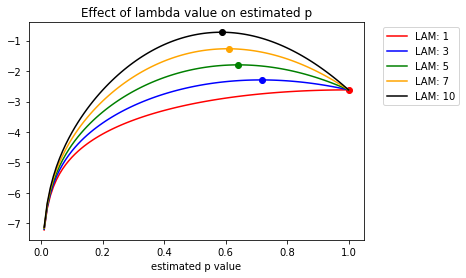
\includegraphics[scale=.75]{./pics/lam-effect.png}
        \caption[Effect of $\lambda$]{Effect of different values of $\lambda$ on estimated $p$ value. The large point on each line is the maximum value, and reflects the returned estimated $p$ of a headline}
        \label{fig:lam-effect}
    \end{center}
\end{figure}

The previous steps give estimators $S$ and $O$. Using these, we are able to estimate the sentiment score $p$ for a new headline that is not in the training sample. Using model \ref{multinom}, we estimate $p$ using Maximum Likelihood Estimation. This is simply testing values in some range and determining which value gives the maximum output. We also include penalty term $\lambda \log(p(1-p))$ and finish with the following optimisation:

\begin{equation}
\widehat p = \arg \max_{p \in [0,1]} \left\{ \widehat s^{-1} \sum_{j \in S} \log (p O_{+,j} + (1-p) O_{-,j}) + \lambda \log(p(1-p)) \right\}
\end{equation}

\noindent
where $\widehat s$ is the total count of word from $S$ in the new headline, $d_j, O_{+,j}, O_{-,j}$ are the entries for word $j$ in the corresponding vectors and $\lambda$ is a tuning parameter that ensures that the majority of headlines are neutral by pushing the estimate towards a neutral sentiment score of 0.5. The effect of lambda is shown in figure \ref{fig:lam-effect}


% \section{Financial Markets and Stock Exchanges}


\section{Portfolios and Financial Market Analysis}
\label{sec:portfolios-analysis}
Evaluating word lists generated by any method of sentiment analysis can be done by creating portfolios based on news with the highest positive or negative sentiment and buying the most positive stocks while selling the negative ones. This gives a good indication of the predictive power of a word list.

\subsection{Portfolios}
\label{sub:portfolios}
A portfolio is simply a list of stocks that can be invested in by an individual or firm. The returns from a portfolio is defined as the profit accrued from all stocks over a set time period, usually daily, monthly or annually. Due to the nature of stocks, simply listing the returns as a concrete value does not convey the information required. For example, if stock `A' were to be invested in at value \$50, and it rose to \$60 the following day, the returns could be said to be \$10. However, if stock `B' were valued at \$1000, and the following day it rose to \$1010, the monetary value would be equivalent at \$10, but the percentage return is vastly different; 20\% returns for stock `A' and 1\% for `B'. For this reason, returns from portfolios are expressed as a percentage.

Daily returns are usually very slight, as the time period is very small, often being smaller than 1\%. In the interest of readability, \textit{basis points} (also known as bps or bips) are used in lieu of a percentage, where 1 bip is equivalent to 0.01\%. This makes it much easier to represent very small returns as are common in daily returns.

\subsubsection{Creating a portfolio}
\label{ssub:portfolio-creation}
A portfolio is constructed using a number of stocks and can be either bought (taking the `long' position) or sold (taking the `short' position). For stocks that are bought, the returns can be calculated from the difference in price at the time that the stock is sold. More concretely, if a stock has value $S_{t}$ at time $t$, and held for $n$ days before being sold, the long returns in percentage form can be calculated using the following formula:

\begin{equation}
\frac{S_{t+n}}{S_{t}} - 1
\end{equation}

\noindent
Similarly, for short returns, as the stock is being sold, profit is acquired if the stock falls in value, therefore the returns can be calculated using the following formula:

\begin{equation}
\frac{S_{t}}{S_{t+n}} - 1
\end{equation}

\noindent
Of course, these simple formulae neglect transaction fees that can apply when constructing real portfolios. However, as we are creating portfolios in a theoretical sense, this suits our needs.

Once the portfolio has been constructed, the weighting for each stock must be considered. Each portfolio will have a value, which is the amount of money invested into it, and each stock will in turn get an investment that is a percentage of this overall value. There are three major strategies that can be used to construct a portfolio: equal weighting, price weighting, and value weighting. Each strategy has its own unique set of advantages and disadvantages.

The equal weighted is perhaps the simplest of these strategies: if a portfolio is comprised of $n$ stocks and has some investment $v$, each stock has $v/n$ invested into it. This strategy glosses over differences in stock size or price.

Price weighted portfolios assign much more money to stocks with higher value associated to them. This can be calculated in a number of ways, but the way we calculate this is if stock $s_i$ in portfolio $P = [s_1, \dots, s_n]$ has market value $P_{i,t}$ at time $t$, the weight of stock $s_i$ would be:

\begin{equation}
w_{i,t} = \frac{P_{i,t}}{\sum_{n}^1 P_{n,t}}
\end{equation}

\noindent
The amount invested into stock $s_i$ at time $t$ would then be $w_{i,t} \times v$.

Finally, value weighted portfolios combine both the price of the stock with the number of outstanding stocks, which creates a much larger bias towards large companies. As before, if stock $s_i$ in portfolio $P=[s_1, \dots, s_n]$ has market value $P_{i,t}$ at time $t$, and has $s_o$ outstanding stocks, the weight of stock $s_i$ is:

\begin{equation}
w_{i,t} = \frac{P_{i,t} \times s_o}{\sum_{n}^1 P_{n,t}}
\end{equation}

Equal weighted stocks more closely resemble hedge funds, as well as being the case that smaller companies are able to more quickly encapsulate market share and investor interest. Equal weighted investments ensure a portfolio has a higher representation of smaller stocks, at the higher risk of the stock failing. Conversely, value weighted portfolios tend to be safer, as they prioritise larger companies that are more stable. The downside to utilising this method is that the large percentage increases observed in smaller stocks will have less effect, and therefore some profit can be lost. Price weighted construction lies somewhere in the middle of the two, being relatively simple to construct, as with equal weighting, but with slight consideration to the price of a stock. The downside of this construction is that the weights assigned are somewhat arbitrary as the price of a stock can fluctuate greatly.

\subsection{Evaluating a portfolio}
To successfully determine the success of a portfolio, it is not always as simple as observing the profit alone. While this is a good indicator of the potential returns that could be gleaned from a given portfolio or investment method, it is important to consider external factors and risks that may be involved. The following methods are used to provide more insight into an investment method.

\subsubsection{Sharpe Ratio}
\label{ssub:sharpe-ratio}
William Sharpe created the Sharpe ratio in 1966 and is one of the most referenced comparison of risk versus return in finance \parencite{sharpe-ratio}. The formula for this ratio is exceedingly simple --- one of the key factors in its wide usage --- and is as follows:

\begin{equation*}
S(x) = \frac{r_x - R_f}{\sigma(r_x)}
\end{equation*}

\noindent
where $x$ is the investment, $r_x$ is the average rate of return of $x$, $R_f$ is the risk free rate of return, and $\sigma(r_x)$ is the standard deviation of $r_x$. The risk free rate of return is simply the theoretical rate of return on an investment with absolutely no risk. Subtracting these risk free returns from the average rate of returns of $x$ yields the true rate of returns.

The value of an investment's Sharpe ratio measures the performance with adjustment for risk: the higher the ratio, the better the performance of the investment when adjusted for risk. As a reference, a ratio of 1 or higher is good, 2 or better is very good, and 3 or better is excellent. 

\subsubsection{Fama French 3 and 5 Factor Models}
\label{ssub:fama-french}
Eugene Fama and Kenneth French co-authored a 1992 paper detailing risk factors in returns on both stocks and bonds. This extends the work Sharpe completed on the Sharpe ratio and goes further in exploring risk factors in returns, along with the capital asset pricing model (CAPM) \parencite{ff3}. CAPM is used for describing systematic risk and expected return, especially for that in stocks. The equation for this is:

\begin{equation}
ER_i = R_f + \beta_t (ER_m - R_f)
\end{equation}

\noindent
where $ER_i$ is the expected return of the investment, $R_f$ is the risk free rate, $\beta_i$ is the beta of the investment and $ER_m - R_f$ is the market risk premium. The beta of an investment is the volatility compared to the rest of the market. It encompasses the sensitivity of a stock to changes in the market. In essence, this gives the expected returns of an asset based on systematic risk. Building on this, Fama and French observed two additional risk factors: the size premium of an asset, or small minus big (SMB), and the value premium, or high minus low (HML). SMB is used to account for companies with small value stocks that generate high returns, while HML accommodates for stocks with equity that is valued cheaply compared to its book value that generate higher returns in comparison to the rest of the market. These factors are used in conjunction to provide the following formula for the Fama French 3 factor model (FF3 model):

\begin{equation*}
ER_i = R_f + \beta_1(ER_m -R_f) + \beta_2 (SMB) + \beta_3(HML) + \alpha
\end{equation*}

The values for SMB and HML are available from French's website \parencite{french_2022}, and can be collected for daily, monthly, or yearly returns. Computing this model on a series of returns from a portfolio gives useful information on the nature of the returns, since the model explains part of the returns. The values for the $\beta$s detail the exposure to each of the risk factors while the $\alpha$, or the intercept, refers to the amount that a portfolio outperformed the expectations of the FF3 model. This alpha is representative of the amount of private or new information that is external from the market and is utilised to construct the portfolio. This means that more simplistic methods of selecting portfolios will not have any private information and therefore the intercept will be much close to zero while a more complicated model will have a larger intercept as simple methods have profits that can be explained by these risk factors.

This model was then revisited by Fama and French in 2015 where they observed two additional factors: robust minus weak (RMW) and conservative minus aggressive (CMA) \parencite{ff5}. RMW corresponds to the profitability of an asset, in that it is the difference between returns of robust or high and weak or low operating profitability. CMA corresponds to the investment factor, and is the difference between returns of conservatively investing firms versus aggressively investing firms, giving the updated formula:

\begin{equation}
ER_i = R_f + \beta_1(ER_m -R_f) + \beta_2 (SMB) + \beta_3(HML) + \beta_4(RMW) + \beta_5(CMA) + \alpha
\end{equation}

%TODO: potentially stick in stuff about momentum factor


% \section{What to do}
% \noindent
% This chapter is intended to describe the background on which execution of the project depends. This may be a technical or a contextual background, or both. The goal is to provide a detailed explanation of the specific problem at hand, and existing work that is relevant (e.g., an existing algorithm that you use, alternative solutions proposed, supporting technologies).  

% Per the same advice in the handbook, note there is a subtly difference from this and a full-blown literature review (or survey).  The latter might try to capture and organise (e.g., categorise somehow) \emph{all} related work, potentially offering meta-analysis, whereas here the goal is simple to ensure the dissertation is self-contained.  Put another way, after reading this chapter a non-expert reader should have obtained enough background to understand what \emph{you} have done (by reading subsequent sections), then accurately assess your work against existing relevant related work.  You might view an additional goal as giving the reader confidence that you are able to absorb, understand and clearly communicate highly technical material and to situate your work within existing literature.







% -----------------------------------------------------------------------------